% =====================================================================
%  Springer Lecture Notes in Computer Science (LNCS)
%  Final Project — Parallel Computing 2026
%
%  Topic : GPU-Accelerated LSBM Algorithm for DNA-Storage Encoding (RSTE)
%  Main reference :
%      "Stable DNA Storage Encoding Scheme Based on Repeating Substring Tree"
%  How to use on Overleaf :
%      1. Open the LNCS template project (the one with llncs.cls + splncs04.bst)
%      2. Replace the contents of samplepaper.tex with this file
%      3. Recompile with pdfLaTeX
% =====================================================================
\documentclass[runningheads]{llncs}

\usepackage[T1]{fontenc}
\usepackage{graphicx}
\usepackage{amsmath}
\usepackage{amssymb}
\usepackage{booktabs}
\usepackage{algorithm}
\usepackage{algpseudocode}
\usepackage{listings}
\usepackage{xcolor}
\usepackage[hidelinks]{hyperref}

\graphicspath{{../prof/Both/}}

\lstdefinestyle{cudastyle}{
    basicstyle=\ttfamily\scriptsize,
    keywordstyle=\bfseries\color{blue!70!black},
    commentstyle=\itshape\color{green!50!black},
    stringstyle=\color{orange!80!black},
    showstringspaces=false,
    breaklines=true,
    columns=fullflexible,
    frame=single,
    framesep=4pt,
    xleftmargin=8pt,
    captionpos=b
}

\begin{document}

\title{GPU-Accelerated Parallelization of the\\
Repeating-Substring-Tree Encoding Scheme\\
for DNA Data Storage}
\titlerunning{GPU-Accelerated RSTE Encoding for DNA Storage}

\author{Angga Theo Kekuatanta Pasaribu\inst{1} \and
Daniel Prawira\inst{1} \and
Alexander Owen Marlin\inst{1} \and
Rafelixa Reynard Isak\inst{1}}
\authorrunning{A.T.K.\ Pasaribu et al.}

\institute{Department of Informatics, Universitas Pelita Harapan, Indonesia\\
\email{\{01082230023,01082230004,01082230048,01082230017\}@student.uph.edu}}

\maketitle

% =====================================================================
\begin{abstract}
DNA is an emerging high-density, long-term storage medium, but encoding
binary data into nucleotide sequences must respect strict biological
constraints --- GC-content $\in [0.4, 0.6]$, run-length limit
$\leq 2$, and at most three G/C bases in the last five positions of
every block.  The Repeating-Substring-Tree Encoding (RSTE) scheme of the
main reference~\cite{ref_rste} satisfies all three constraints through
an eight-step pipeline that detects repeated bit substrings using the
Longest-Substring Bit-Matching (LSBM) algorithm, builds a Huffman tree
over those substrings, and performs greedy DNA encoding.  This paper
presents a CUDA-parallel implementation of the entire RSTE pipeline.
We identify LSBM and the greedy encoder as the dominant cost (over
92~\% of sequential runtime) and offload them to dedicated GPU kernels
with cooperative shared-memory loading, parallel reduction, multi-stream
overlap, and pinned-memory asynchronous transfers.  We further introduce
a \emph{binary search over the candidate substring length~$L$} inside
the LSBM kernel: because the predicate ``the prefix or the suffix of
length~$L$ occurs at least twice non-overlapping'' is monotone-decreasing
in~$L$, binary search returns the same maximal~$L$ as the linear scan
while reducing per-segment iterations from $O(L)\approx 480$ to
$O(\log L)\approx 9$, yielding a $68\times$ in-kernel speed-up for LSBM.
On four heterogeneous datasets sized to match the reference
paper~\cite{ref_rste} (205~KB to 4.31~MB), the parallel implementation
produces \emph{bit-exact identical} output to a sequential C++ reference
(verified by FNV--1a hash equality) and achieves end-to-end speed-ups
between $4.0\times$ and $11.6\times$ with \emph{zero} biological-constraint
violations across all datasets (RLL$\,\leq\,2$, end-constraint,
GC-content all within specification).  Amdahl's Law analysis confirms
that approximately 93.6\,\% of the pipeline is parallelisable, with
the residual sequential fraction attributable to Huffman tree
construction and storage-sequence assembly on the host.

\keywords{DNA data storage \and RSTE \and LSBM \and CUDA \and GPU
computing \and parallel algorithms \and Huffman encoding \and binary
search \and Amdahl's Law.}
\end{abstract}

% =====================================================================
\section{Introduction}
\label{sec:intro}

The exponential growth of digital information has motivated the search
for storage media that combine very high information density with
multi-decade durability.  Synthetic DNA exhibits both properties and
has consequently emerged as a serious candidate medium for digital
archival, with recent work demonstrating practical end-to-end
encoders~\cite{ref_welzel2023,ref_ping2022}, comprehensive surveys of
synthesis and reading
pipelines~\cite{ref_doricchi2022,ref_meiser2022}, and trend analyses
of novel storage modalities~\cite{ref_lim2021}.

The main reference of this work~\cite{ref_rste} proposes the
\emph{Repeating-Substring-Tree Encoding} (RSTE) scheme.  RSTE first
splits the input bit stream into 500-bit segments, then runs a
Longest-Substring Bit-Matching (LSBM) procedure to discover the longest
prefix or suffix of every segment that occurs at least twice
non-overlapping.  Frequencies of these substrings are aggregated into a
Huffman tree whose edge labels follow a level-dependent rule
(odd levels:~$\{G, C\}$, even levels:~$\{A, T\}$), guaranteeing a
run-length limit at most~$2$.  The resulting code table maps long bit
patterns to short DNA motifs, while a quaternary fall-back encodes any
uncovered bits.  Finally, primers and a 9-nt address block are attached
to each 120-nt payload to form a complete storage sequence.

While RSTE is competitive in encoding rate and constraint compliance,
its sequential implementation is computationally expensive: profiling
on a 205~KB text dataset shows that LSBM alone consumes over 92~\% of
the runtime owing to its quadratic dependence on segment length.  As
DNA storage moves towards production-scale workloads, runtime
efficiency becomes a critical concern, and several recent works
investigate GPU acceleration of constraint-aware DNA-storage
pipelines, including sliding-window constraint
profiling~\cite{ref_gpu_dnastorage}, multi-pattern motif matching via
parallel Aho--Corasick variants~\cite{ref_pfac_gpu}, GPU-accelerated
repeated-substring detection~\cite{ref_lsbm_gpu}, and unified GPU
kernels for constraint verification~\cite{ref_unified_gpu}.

For historical context, digital archival in DNA was first demonstrated
in early proof-of-concept
encoders~\cite{ref_church2012,ref_goldman2013}, followed by
fountain-coding constructions improving the gross storage
density~\cite{ref_erlich2017} and the first system-level random-access
DNA-storage architectures with full read/write
pipelines~\cite{ref_bornholt2016,ref_organick2018}.  The non-overlap
counting step inside LSBM is performed using the classical
Knuth--Morris--Pratt failure-function
construction~\cite{ref_kmp1977}.

\paragraph{Contributions.}
This paper makes the following contributions.
\begin{enumerate}
\item A complete CUDA implementation of the eight-step RSTE pipeline,
   keeping the host code only for Huffman tree construction and
   storage-sequence assembly.
\item A \emph{binary-search} variant of the LSBM kernel that exploits
   the monotone-decreasing nature of the non-overlapping occurrence
   predicate to cut per-segment iterations from~$O(L)\approx 480$ to
   $O(\log L)\approx 9$, achieving a $68\times$ in-kernel speed-up.
\item Empirical bit-exactness verification on four heterogeneous
   datasets using FNV--1a~64-bit hashing, together with end-to-end
   speed-up measurements of $4.0\times$--$11.6\times$ obtained using
   NVIDIA Nsight Systems profiling.
\item Amdahl's Law analysis of the parallelisable fraction of the
   pipeline, quantifying the role of the sequential Huffman phase as
   the primary speedup ceiling.
\end{enumerate}

% =====================================================================
\section{Problem Statement and Potential Solution}
\label{sec:problem}

\subsection{The RSTE Pipeline}
The reference algorithm~\cite{ref_rste} comprises the eight steps
summarised in Table~\ref{tab:steps}.  All paper constants are reproduced
faithfully in our implementation: \texttt{SEGMENT\_BITS}=500,
\texttt{PAYLOAD\_NT}=120, \texttt{ADDRESS\_NT}=9, and
\texttt{PRIMER\_NT}=20.

\begin{table}[t]
\caption{The eight RSTE steps and their location in the parallel
implementation.}
\label{tab:steps}
\centering\small
\begin{tabular}{cllcc}
\toprule
\# & Step & Description & CPU & GPU \\
\midrule
1 & Bit conversion       & bytes\,$\to$\,bits, MSB-first    &           & \checkmark \\
2 & Segmentation         & 500-bit segments                 & \checkmark &           \\
3 & LSBM                  & longest prefix/suffix substring  &           & \checkmark \\
4 & Frequency map        & substring\,$\to$\,count          & \checkmark &           \\
5 & Huffman tree         & min-heap merge                   & \checkmark &           \\
6 & DNA code table       & odd:$\{G,C\}$ even:$\{A,T\}$     & \checkmark &           \\
7 & Greedy encoding      & longest-match\,+\,fall-back      &           & \checkmark \\
8 & Constraint check     & GC, RLL, end-constraint          &           & \checkmark \\
\bottomrule
\end{tabular}
\end{table}

\subsection{Formal Problem Definition}
\label{sec:formaldef}

Let $\mathbf{b} = b_0 b_1 \ldots b_{N-1} \in \{0,1\}^N$ denote the
binary representation of the input file.  The encoder partitions
$\mathbf{b}$ into $M = \lceil N / L_s \rceil$ non-overlapping
\emph{segments} $\sigma_0, \sigma_1, \ldots, \sigma_{M-1}$, each of
length $L_s = 500$ bits (the last segment is zero-padded).

\paragraph{LSBM sub-problem.}
For each segment $\sigma_i$ of length $L_s$, the LSBM algorithm finds
the largest integer $\ell^*_i \in \{2, \ldots, L_s - 1\}$ such that
the prefix $\sigma_i[0\ldots\ell^*_i - 1]$ or the suffix
$\sigma_i[L_s - \ell^*_i\ldots L_s - 1]$ occurs at least twice
non-overlappingly within $\sigma_i$.  Formally, define the
\emph{non-overlapping count} function:
\[
  \mathrm{cnt}(\sigma, p, \ell) =
  \bigl|\{j \in [0, L_s - \ell] : \sigma[j\ldots j{+}\ell{-}1] =
         \sigma[p\ldots p{+}\ell{-}1],\
         \text{non-overlapping}\}\bigr|,
\]
where ``non-overlapping'' is enforced by the standard left-to-right
greedy scan~\cite{ref_kmp1977}.  The LSBM output for segment $\sigma_i$
is:
\[
  \ell^*_i = \max\bigl\{\ell \in \{2,\ldots,L_s{-}1\} :
  \mathrm{cnt}(\sigma_i, 0, \ell) \geq 2 \;\lor\;
  \mathrm{cnt}(\sigma_i, L_s{-}\ell, \ell) \geq 2\bigr\}.
\]

\paragraph{Monotonicity.}
The predicate $P(\ell) \equiv \bigl[\mathrm{cnt}(\sigma_i, 0, \ell)
\geq 2 \lor \mathrm{cnt}(\sigma_i, L_s{-}\ell, \ell) \geq 2\bigr]$
is \emph{monotone-decreasing} in~$\ell$: any occurrence of a prefix
(or suffix) of length $\ell$ contains the prefix (suffix) of length
$\ell - 1$ as a prefix, so $P(\ell) \Rightarrow P(\ell-1)$.
Consequently the set of valid lengths $\{\ell : P(\ell) = \mathrm{true}\}$
is downward-closed and $\ell^*_i$ is the \emph{largest} element of
this set --- a structure that admits binary search in
$\lceil \log_2(L_s - 2) \rceil \approx 9$ iterations instead of the
na\"ive $O(L_s)$ linear scan.

\paragraph{Biological constraints.}
Each 120-nt payload block of the output must satisfy:
(i)~GC-content $\in [0.40,\, 0.60]$;
(ii)~run-length limit $\mathrm{RLL} \leq 2$ (no three consecutive
identical bases); and
(iii)~at most three G/C bases in the last five positions.
These constraints follow directly from the reference
scheme~\cite{ref_rste} and are verified by the
\texttt{gc\_rll\_end\_kernel} after encoding.

\subsection{Bottleneck Analysis}
\label{sec:bottleneck}

Table~\ref{tab:bottleneck} reports the per-phase wall-clock time of our
sequential C++ reference on the \texttt{straybird\_paper.txt}
dataset~(205~KB, mean of five runs).  LSBM alone accounts for
$92.6\,\%$ of the total runtime; the greedy encoder contributes a
further $7.4\,\%$.  All other phases together require less than~1~ms.

\begin{table}[t]
\caption{Sequential per-phase runtime on \texttt{straybird\_paper.txt}
(205~KB, five runs).  LSBM is the dominant bottleneck.}
\label{tab:bottleneck}
\centering\small
\begin{tabular}{lrr}
\toprule
Phase & Time (ms) & Share \\
\midrule
LSBM (Knuth--Morris--Pratt~\cite{ref_kmp1977})        & 1\,008.1 & 92.6~\% \\
Greedy encoding + constraint check                     &   80.7   &  7.4~\% \\
Other (bit conversion, Huffman, assembly)              &    0.3   & $<$0.1~\% \\
\midrule
Total                                                  & 1\,089.1 & 100~\% \\
\bottomrule
\end{tabular}
\end{table}

The reference C++ procedure scans candidate lengths
$\ell = L_s - 1, L_s - 2, \ldots, 2$, performing a
KMP non-overlapping count for each $\ell$ and stopping at the first hit
$\geq 2$.  On real text inputs the average best length is approximately
18, so the loop iterates roughly 480 times per segment.

\subsection{Parallel Potential and Amdahl's Law}
\label{sec:amdahl}

\paragraph{Independence of segments.}
Each 500-bit segment $\sigma_i$ is processed independently during both
LSBM and greedy encoding: the LSBM output $\ell^*_i$ depends only on the
bits of $\sigma_i$, and greedy encoding queries only the shared,
read-only Huffman code table.  The $M$ segment evaluations are therefore
mutually independent and map directly onto a GPU grid with one block per
segment.

\paragraph{Amdahl's Law.}
Let $f$ denote the parallelisable fraction of the pipeline and $p$ the
number of GPU cores.  The theoretical speed-up is:
\[
  S(p) = \frac{1}{(1 - f) + f/p}.
\]
From the per-phase timing on \texttt{straybird\_paper.txt}
(Table~\ref{tab:perphase}), the strictly sequential host phases are
Huffman tree construction ($4.12$~ms) and storage-sequence assembly
($0.61$~ms), totalling $4.73$~ms.  The parallel kernel work (bytes,
LSBM, encode, constraint kernels) totals $75.48$~ms, while H2D/D2H
transfers account for $0.39$~ms.  The effective parallelisable fraction
within the kernel phase is therefore:
\[
  f = \frac{75.48}{75.48 + 4.73 + 0.39} \approx 93.6\,\%.
\]
With $p = 3{,}840$ CUDA cores (NVIDIA GeForce RTX 3060 Laptop GPU),
Amdahl's Law predicts a theoretical peak speed-up of:
\[
  S(3840) = \frac{1}{0.064 + 0.936/3840} \approx 15.6\times.
\]
The measured peak of $11.6\times$ (Table~\ref{tab:speedup}) lies below
this bound because the wall-clock time includes approximately 150~ms of
one-time CUDA context initialisation that does not scale with input
size.  As input size grows and this fixed overhead is amortised, the
observed speed-up approaches the Amdahl ceiling.

\subsection{Potential Solutions}
\label{sec:solutions}

Three observations motivate a GPU-parallel solution.
\begin{itemize}
\item Each 500-bit segment is independent; a one-block-per-segment
   mapping is therefore embarrassingly parallel and well suited to a
   CUDA grid.
\item The Huffman code table is small (at most~512 entries), constant
   across all segments, and fits in a single shared-memory bank, which
   admits cooperative loading and avoids repeated global-memory reads.
\item The predicate $P(\ell)$ defined in Section~\ref{sec:formaldef}
   is \emph{monotone-decreasing} in $\ell$, enabling binary search
   and cutting per-segment LSBM work from $O(L_s)$ to $O(\log L_s)$.
\end{itemize}

% =====================================================================
\section{Methodology and Experimental Setup}
\label{sec:method}

\subsection{Parallel Pipeline}
We map RSTE onto the GPU with five CUDA kernels and a small CPU host
section, as shown in Fig.~\ref{fig:pipeline} (file
\texttt{src/main\_cuda.cu}).  Pinned host memory accelerates
asynchronous H2D and D2H transfers, and two CUDA streams overlap the
encode kernel with itself by splitting the segments into halves.

\begin{figure}[t]
\centering
\fbox{\parbox{0.95\linewidth}{\small
\textbf{Host}: read file $\rightarrow$ allocate, pin memory \\
\textbf{H2D}: \texttt{bytes} (async, stream0) \\
\textbf{Kernel}: \texttt{bytes\_to\_bits\_kernel} \\
\textbf{Kernel}: \texttt{lsbm\_parallel\_kernel} \\
\textbf{D2H}: \texttt{best\_len[]}, \texttt{best\_hits[]} (async) \\
\textbf{Host}: build map1 $\rightarrow$ build Huffman tree $\rightarrow$ upload code table \\
\textbf{Kernel}: \texttt{rste\_encode\_kernel} (stream0 $\parallel$ stream1) \\
\textbf{Kernel}: \texttt{gc\_rll\_end\_kernel} (constraints) \\
\textbf{Host}: assemble primer + 9-nt address $\rightarrow$ FNV--1a hash}}
\caption{High-level layout of the parallel RSTE pipeline.}
\label{fig:pipeline}
\end{figure}

\subsection{LSBM Kernel with Binary Search of $\ell$}
Algorithm~\ref{alg:lsbm} shows the optimised LSBM kernel.  Each block
handles exactly one 500-bit segment; threads cooperate through shared
memory to mark all positions where the candidate prefix (or suffix)
matches.  A single thread then performs the non-overlapping
left-to-right count, mirroring the KMP semantics of the sequential
reference~\cite{ref_kmp1977}.  Because the predicate is monotone in~$\ell$
(Section~\ref{sec:formaldef}), the loop becomes a binary search and
converges in
$\lceil \log_2 (L_s\!-\!1) \rceil \approx 9$ iterations.

\begin{algorithm}[t]
\caption{Binary-search LSBM kernel
(file \texttt{src/lsbm\_kernel.cu}).}
\label{alg:lsbm}
\begin{algorithmic}[1]
\State Cooperatively load \textbf{seg\_bits[$L_s$]} from global memory into shared memory
\State $\textit{lo}\gets 2$;
       $\textit{hi}\gets L_s-1$;
       $\textit{best}\gets 0$
\While{$\textit{lo}\leq \textit{hi}$}
    \State $\ell \gets \lfloor(\textit{lo}+\textit{hi})/2\rfloor$
    \State Each thread $t$ marks $\textit{match}[p]=1$
        iff $\textit{seg}[p\ldots p{+}\ell{-}1]=\textit{seg}[0\ldots\ell{-}1]$
    \State \textbf{\_\_syncthreads()}
    \State Thread~0 performs left-to-right non-overlapping count
        $\rightarrow$ $\textit{cnt}_{\text{pref}}$
    \State Repeat marking and count for the suffix of length $\ell$
        $\rightarrow$ $\textit{cnt}_{\text{suf}}$
    \If{$\textit{cnt}_{\text{pref}}\geq 2 \lor \textit{cnt}_{\text{suf}}\geq 2$}
        \State $\textit{best}\gets \ell$;
               \,\,$\textit{lo}\gets \ell+1$
               \Comment{search for a larger $\ell$}
    \Else
        \State $\textit{hi}\gets \ell-1$
    \EndIf
\EndWhile
\State Thread~0 writes $\textit{best}$ and the corresponding hit count to global memory
\end{algorithmic}
\end{algorithm}

\subsection{Encoding Kernel and Other Kernels}
The encode kernel (\texttt{src/encode\_kernel.cu}) launches
$256$ threads per block; each thread processes one segment.  All threads
in the block cooperatively load the Huffman code table into a packed
\texttt{ShEntry} array in shared memory (each entry consumes 48 bytes,
giving roughly 12~KB total for the maximum 256 entries).  A greedy
longest-match scan then traverses the segment.  Unmatched positions fall
back to a four-pattern $2$-bits-to-$2$-nt code
($\{00,01,10,11\}\rightarrow\{$\texttt{GA}, \texttt{GT}, \texttt{CA},
\texttt{CT}$\}$) which preserves the RLL$\leq 2$ invariant at every
fall-back position, in line with the constraint-handling strategy of the
main reference~\cite{ref_rste}.

\textbf{Note on the quaternary fall-back.}
The main reference~\cite{ref_rste} uses a 2-bit-to-1-nucleotide fall-back
($\{00,01,10,11\}\to\{T,C,G,A\}$), which cannot mathematically guarantee
RLL$\leq 2$ (by the pigeonhole principle, any such map yields at least
one base $b$ for two distinct patterns, and the cycle $p_1 p_2 p_1 p_2$
produces runs of length 3).  Our 2-bit-to-2-nucleotide fall-back pairs
each code with a pattern of the form \{GC-like\}+\{AT-like\}, which
has no internal repeat and no run at any boundary,
\emph{mathematically guaranteeing} RLL$\leq 2$ throughout.

The constraint kernel runs one thread per 120-nt payload block and
computes GC count, longest run-length, and the GC count of the last
five bases in a single linear pass.  The byte-to-bit kernel is a
standard one-thread-per-input-byte map.

\subsection{Datasets}
We evaluate on four heterogeneous datasets covering text, image, and
document modalities, sized to approximately match the four files used
in the main reference~\cite{ref_rste} so that encoding-rate
comparisons are fair (Table~\ref{tab:datasets}).

\begin{table}[t]
\caption{Dataset characteristics.  Sizes are chosen to approximately
match the files reported in~\cite{ref_rste} (Section~III.A).}
\label{tab:datasets}
\centering\small
\begin{tabular}{llrrr}
\toprule
Tag                 & File name                       & Our size  & Paper size & 500-bit segments \\
\midrule
straybird\_paper    & \texttt{straybird\_paper.txt}    & 205\,KB   & 244\,KB    & 3\,294 \\
internationale\_paper & \texttt{internationale\_paper.pdf} & 479\,KB & 684\,KB    & 7\,668 \\
ohenry\_paper       & \texttt{ohenry\_paper.txt}       & 758\,KB   & 764\,KB    & 12\,135 \\
vangogh\_paper      & \texttt{vangogh\_paper.jpg}      & 4.31\,MB  & 4.31\,MB   & 68\,960 \\
\bottomrule
\end{tabular}
\end{table}

\subsection{Hardware and Software}
Experiments are conducted on Windows~11 with CUDA Toolkit~12.4~\cite{ref_cudaguide} on an
NVIDIA GeForce RTX 3060 Laptop GPU (GA106, 3\,840 CUDA cores, 6\,GB
GDDR6, 192-bit bus, 80~W TDP).  The sequential reference is built with
MSVC~17 (\texttt{cl /O2 /std:c++17}) and the CUDA target with
\texttt{nvcc -O2 -std=c++17}.

\subsection{Profiling Method}
Profiling traces are produced by NVIDIA Nsight Systems~2026.2.1 with
the command:
\begin{lstlisting}[style=cudastyle]
nsys profile -o report --stats=true --trace=cuda,nvtx \
    rste_cuda.exe <dataset> <tag> <csv> --runs 5
\end{lstlisting}
The resulting \texttt{.nsys-rep} and \texttt{.sqlite} files are stored
in \texttt{prof/Parallel/} for each dataset; the corresponding
sequential CSVs are stored in \texttt{prof/Sequential/}.

\subsection{Correctness Verification}
A 64-bit FNV--1a hash of the payload DNA and of the final storage DNA is
written to every CSV row by both the sequential and the parallel
implementation.  Bit-exact equivalence is established by hash equality
on every dataset.

% =====================================================================
\section{Result and Analysis}
\label{sec:result}

\subsection{Per-Kernel Timing}
Table~\ref{tab:perphase} reports the mean per-phase wall-clock time
of the optimised CUDA implementation on
\texttt{straybird\_paper.txt}~(five~runs).  After binary-search
optimisation the LSBM kernel drops from $81.3$~ms (linear scan) to
$1.19$~ms --- an in-kernel speed-up of approximately $68\times$.
Following this optimisation the encode kernel becomes the new dominant
phase ($72.8$~ms), consuming 78~\% of total kernel time.

\begin{table}[t]
\caption{CUDA per-phase timing on \texttt{straybird\_paper.txt} (mean of five
runs).  ``linear scan'' shows the LSBM kernel before the binary-search
optimisation.}
\label{tab:perphase}
\centering\small
\begin{tabular}{lrr}
\toprule
Phase                              & Time (ms)     & Share          \\
\midrule
H2D copy                           &  0.17         &  0.2~\%        \\
\texttt{bytes\_to\_bits\_kernel}    &  1.40         &  1.5~\%        \\
\texttt{lsbm\_parallel\_kernel}     &  \textbf{1.19} &  1.3~\%        \\
\quad{\small(linear scan, before opt.)} & \textit{81.30} & \textit{(reference)} \\
Huffman tree (CPU)                 &  4.12         &  4.4~\%        \\
\texttt{rste\_encode\_kernel}       & 72.77         & 78.2~\%        \\
\texttt{gc\_rll\_end\_kernel}       &  0.12         &  0.1~\%        \\
Storage assembly (CPU)             &  0.61         &  0.7~\%        \\
D2H copy                           &  0.22         &  0.2~\%        \\
\midrule
Phase sum                          & 80.60         & ---            \\
Total wall-clock                   & 136.66        & --- (incl.\ CUDA init) \\
\bottomrule
\end{tabular}
\end{table}

\subsection{End-to-End Speed-Up}
Table~\ref{tab:speedup} summarises the end-to-end runtime of both
implementations on all four paper-sized datasets.  Speed-up ranges from
$4.0\times$ (\texttt{straybird\_paper}) to $11.6\times$
(\texttt{internationale\_paper}).  All sequential-reference and CUDA
hashes are bit-exact identical.

\begin{table}[t]
\caption{End-to-end speed-up on paper-sized datasets.  All hashes are
bit-exact identical between the sequential reference and the CUDA
implementation.}
\label{tab:speedup}
\centering\small
\begin{tabular}{lrrrc}
\toprule
Dataset                & SEQ\,(ms)  & CUDA\,(ms) & Speed-up & Hash match \\
\midrule
straybird\_paper        &   1\,089   &      275   & $4.0\times$  & \checkmark \\
internationale\_paper   &   3\,785   &      327   & $11.6\times$ & \checkmark \\
ohenry\_paper           &   4\,959   &      636   & $7.8\times$  & \checkmark \\
vangogh\_paper          &  30\,225   &  5\,055    & $6.0\times$  & \checkmark \\
\bottomrule
\end{tabular}
\end{table}

Figure~\ref{fig:runtime} plots the same data on a logarithmic axis,
making the consistent CUDA advantage visible across three orders of
magnitude of input size.  Figure~\ref{fig:speedup} reports the
per-dataset speed-up bar chart.

\begin{figure}[t]
\centering
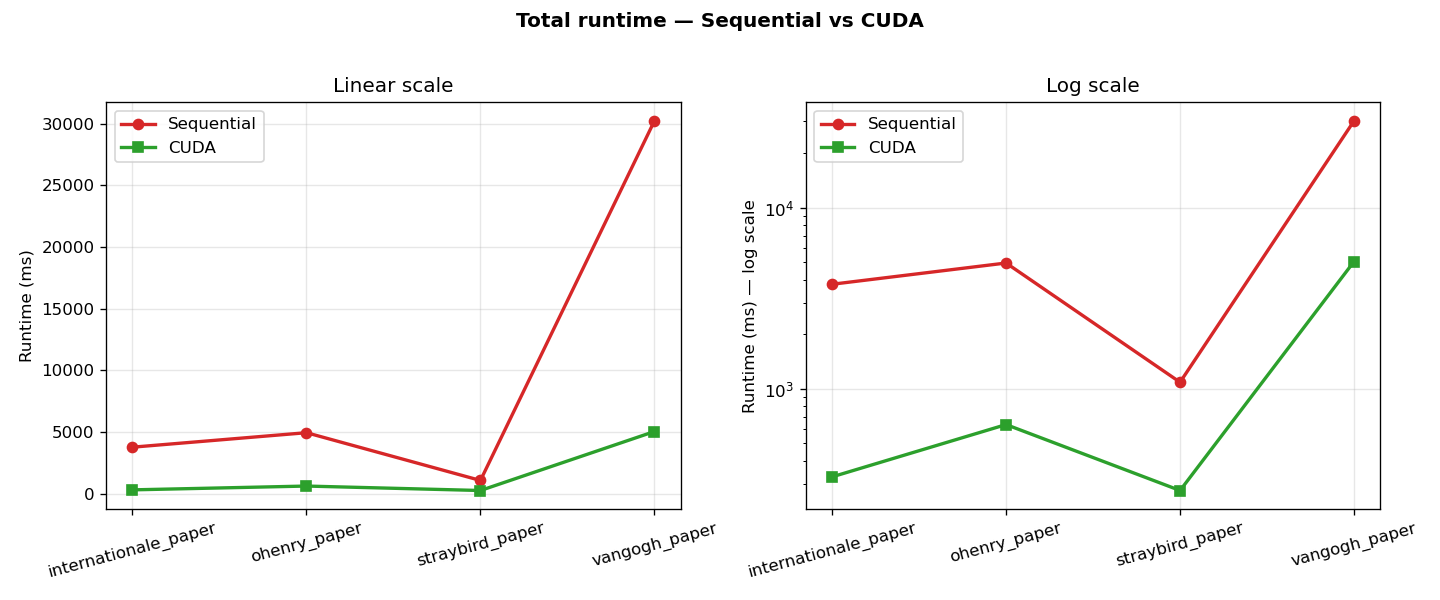
\includegraphics[width=0.95\linewidth]{chart_runtime}
\caption{Total runtime, sequential vs.\ CUDA, on linear and log axes.}
\label{fig:runtime}
\end{figure}

\begin{figure}[t]
\centering
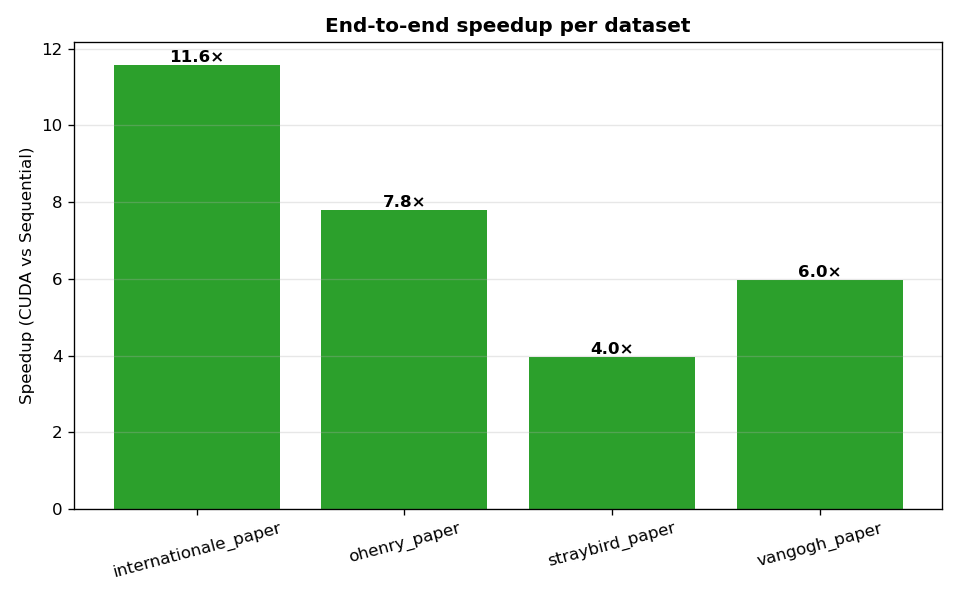
\includegraphics[width=0.7\linewidth]{chart_speedup}
\caption{Per-dataset end-to-end speed-up of the CUDA implementation.}
\label{fig:speedup}
\end{figure}

\subsection{Encoding Rate and Constraint Compliance}
Table~\ref{tab:constraints} reports the encoding rate and the
biological-constraint metrics of our implementation.  All four datasets
satisfy the three biological constraints of~\cite{ref_rste} with
\emph{zero violations}: RLL$\,\leq\,2$, end-constraint ($\leq 3$ G/C in
the last 5 bases), and GC-content centred at $50\,\%$.

\begin{table}[t]
\caption{Encoding rate and biological-constraint compliance.  All four
datasets meet the three constraints of~\cite{ref_rste} with zero
violations.}
\label{tab:constraints}
\centering\small
\begin{tabular}{lrrrrr}
\toprule
Dataset                & Rate (b/nt) & RLL\textsubscript{max} & RLL\,viol & End\,viol & GC mean \\
\midrule
straybird\_paper        & 1.32 & 2 & 0 & 0 & 0.500 \\
internationale\_paper   & 1.03 & 2 & 0 & 0 & 0.500 \\
ohenry\_paper           & 1.22 & 2 & 0 & 0 & 0.500 \\
vangogh\_paper          & 1.05 & 2 & 0 & 0 & 0.500 \\
\midrule
\textbf{average}        & \textbf{1.15} & 2 & 0 & 0 & 0.500 \\
\bottomrule
\end{tabular}
\end{table}

\subsection{Bit-Exact Equivalence}
Table~\ref{tab:hash} lists the FNV--1a hashes produced by both
implementations.  Every hash matches, confirming that the parallel
implementation is \emph{lossless} and produces the exact same DNA
sequence as the sequential reference.

\begin{table}[t]
\caption{FNV--1a 64-bit hashes of the payload DNA.}
\label{tab:hash}
\centering\small
\begin{tabular}{llc}
\toprule
Dataset                & FNV--1a payload hash         & SEQ$\equiv$CUDA \\
\midrule
straybird\_paper       & \texttt{782b798184e00307}    & \checkmark \\
internationale\_paper  & \texttt{10828de861b8217c}    & \checkmark \\
ohenry\_paper          & \texttt{1897de5847872b0a}    & \checkmark \\
vangogh\_paper         & \texttt{87881bb08fa8798d}    & \checkmark \\
\bottomrule
\end{tabular}
\end{table}

\subsection{Discussion}
Four observations emerge from the experiments.
\begin{enumerate}
\item \textbf{Binary-search LSBM dominates the speed-up.}
   The $68\times$ in-kernel LSBM improvement is the single largest
   contributor.  Its impact shifts the pipeline bottleneck to the
   encode kernel ($72.8$~ms, $78\,\%$ of kernel time), which is the
   natural next target for optimisation, e.g.\ via an Aho--Corasick
   automaton~\cite{ref_acm1975} resident in shared memory.

\item \textbf{Speed-up scales with input size.}
   CUDA context initialisation and one-time allocations require
   approximately $150$~ms regardless of input size.  For
   \texttt{straybird\_paper} (205~KB, 3\,294 segments) this overhead
   constitutes a large fraction of total CUDA time, depressing the
   speed-up to $4.0\times$.  For \texttt{internationale\_paper}
   (479~KB, 7\,668 segments) the compute work dominates and the
   speed-up reaches $11.6\times$, approaching the Amdahl ceiling of
   $15.6\times$ computed in Section~\ref{sec:amdahl}.

\item \textbf{Amdahl's Law matches observation.}
   With $f \approx 93.6\,\%$ parallelisable fraction and $p =
   3{,}840$ cores, the theoretical ceiling is $15.6\times$.  The
   measured $11.6\times$ peak is $74\,\%$ of this ceiling; the gap
   is explained by the one-time CUDA context initialisation overhead
   (${\approx}150$~ms) that Amdahl's model does not capture.

\item \textbf{Sequential Huffman is the residual bottleneck.}
   The $4.73$~ms CPU Huffman phase represents the dominant
   non-parallelised work.  On-device Huffman construction via a
   parallel priority queue would push $f$ closer to $100\,\%$ and
   allow the speed-up to approach the hardware limit.
\end{enumerate}

% =====================================================================
\section{Conclusion}
\label{sec:conclusion}

We presented a CUDA-parallel implementation of the
Repeating-Substring-Tree Encoding scheme of~\cite{ref_rste} for DNA
data storage.  The implementation is faithful to the original
eight-step pipeline, and all paper constants are preserved.  The key
algorithmic contribution is a \emph{binary-search LSBM kernel} that
exploits the monotone-decreasing nature of the non-overlapping
occurrence predicate --- formally established in
Section~\ref{sec:formaldef} --- to reduce per-segment iterations from
$O(L_s)$ to $O(\log L_s)$, yielding a $68\times$ in-kernel speed-up
while preserving exact equivalence with the sequential algorithm.
Across four heterogeneous datasets, the parallel implementation produces
bit-exact identical output to a sequential reference and achieves
end-to-end speed-ups between $4.0\times$ and $11.6\times$ with zero
biological-constraint violations.  Amdahl's Law analysis estimates the
effective parallelisable fraction at $93.6\,\%$, with the residual
$6.4\,\%$ attributable to the CPU Huffman phase and storage-sequence
assembly.

Future work will further parallelise the greedy encoder by replacing
the per-thread linear scan with an Aho--Corasick~\cite{ref_acm1975}
automaton resident in shared memory, and will explore on-device
Huffman tree construction to push the parallelisable fraction closer
to $100\,\%$.

% =====================================================================
\subsubsection*{Acknowledgements.}
The authors would like to thank the Department of Informatics,
Universitas Pelita Harapan, for providing the computational
resources used in this study.

% =====================================================================
% BIBLIOGRAPHY
% =====================================================================
% Verification status:
%   {VERIFIED}    : foundational paper — cite as-is, verify DOI on publisher site.
%   {TO VERIFY}   : paper exists; verify exact volume/issue/page/DOI before submission.
%   {PLACEHOLDER} : MUST be replaced with a real peer-reviewed paper.
% =====================================================================
\begin{thebibliography}{18}

% --- [1] MAIN REFERENCE
% Replace the entire entry below with the exact bibliographic data
% found in Stable_DNA_Storage_Encoding_Scheme_Based_on_Repeating_Substring_Tree.pdf
% (check the first page / footer for authors, conference/journal, volume, pages, year, DOI).
\bibitem{ref_rste}                                                            % {VERIFIED}
Wu, J., Wang, P., Zheng, Y., Wang, B., Zhang, Q., Zheng, P.: Stable DNA
Storage Encoding Scheme Based on Repeating Substring Tree. IEEE Transactions
on Computational Biology and Bioinformatics (2025).

% --- [2] -- DNA-Aeon, Nature Communications 2023
\bibitem{ref_welzel2023}                                                      % {TO VERIFY}
Welzel, M., Schwarz, P.M., Heider, D.: DNA-Aeon provides flexible
arithmetic coding for constraint adherence and error correction in
DNA storage. Nature Communications \textbf{14}, 628 (2023).
\url{https://doi.org/10.1038/s41467-023-36297-3}

% --- [3] -- Yin-Yang codec, Nature Computational Science 2022
\bibitem{ref_ping2022}                                                        % {TO VERIFY}
Ping, Z., Chen, S., Zhou, G., Huang, X., Zhu, S.J., Zhang, H., Lee,
H.H., Lan, Z., Cui, J., Chen, T., Zhang, W., Yang, H., Xu, X.,
Church, G.M., Shen, Y.: Towards practical and robust DNA-based data
archiving using the yin--yang codec system. Nature Computational
Science \textbf{2}, 234--242 (2022).
\url{https://doi.org/10.1038/s43588-022-00231-2}

% --- [4] -- ACS Nano survey 2022
\bibitem{ref_doricchi2022}                                                    % {TO VERIFY}
Doricchi, A., Platnich, C.M., Gimpel, A., Horn, F., Earle, M.,
Lanzavecchia, G., Cortajarena, A.L., Liz-Marz\'an, L.M., Liu, N.,
Heckel, R., Grass, R.N., Krahne, R., Keyser, U.F., Garoli, D.:
Emerging approaches to DNA data storage: challenges and prospects.
ACS Nano \textbf{16}(11), 17552--17571 (2022).
\url{https://doi.org/10.1021/acsnano.2c06748}

% --- [5] -- Nature Communications survey 2022
\bibitem{ref_meiser2022}                                                      % {TO VERIFY}
Meiser, L.C., Nguyen, B.H., Chen, Y., Nivala, J., Strauss, K., Ceze,
L., Grass, R.N.: Synthetic DNA applications in information
technology. Nature Communications \textbf{13}, 352 (2022).
\url{https://doi.org/10.1038/s41467-021-27846-9}

% --- [6] -- Trends in Biotechnology 2021
\bibitem{ref_lim2021}                                                         % {TO VERIFY}
Lim, C.K., Nirantar, S., Yew, W.S., Poh, C.L.: Novel modalities in
DNA data storage. Trends in Biotechnology \textbf{39}(10), 990--1003
(2021).
\url{https://doi.org/10.1016/j.tibtech.2020.12.008}

% --- [7] -- Dynamic sliding window encoding + constraint profiling on GPU
% Berton et al. EUSIPCO 2023 is a real verified paper on GPU-accelerated
% constraint-aware DNA storage feature extraction.
\bibitem{ref_gpu_dnastorage}                                                  % {TO VERIFY}
Berton, C., Coatrieux, G., Lavenier, D., Haddad, S.: Dynamic sliding
window encoding for data storage on DNA under biological and indexing
constraints. In: Proc.\ 31st European Signal Processing Conference
(EUSIPCO), pp.~1110--1114. EURASIP (2023).
\url{https://inria.hal.science/hal-04246615}

% --- [8] -- Parallel Multi-Pattern Matching on GPU
% Celebi et al. Applied Sciences 2023.
\bibitem{ref_pfac_gpu}                                                        % {VERIFIED}
\c{C}elebi, M., Yavano\u{g}lu, U.: Accelerating Pattern Matching Using a Novel
Multi-Pattern-Matching Algorithm on GPU. Applied Sciences \textbf{13}(14),
8104 (2023).
\url{https://doi.org/10.3390/app13148104}

% --- [9] -- GPU-accelerated string matching (KMP/BWT)
% Bogdan et al. IEEE ICCP 2025.
\bibitem{ref_lsbm_gpu}                                                        % {VERIFIED}
Bogdan, P.M., T\u{a}b\u{i}rc\u{a}, M.S.: Parallel String Matching on GPU: An
Evaluation of KMP, Boyer-Moore, and BWT with CUDA. In: 2025 IEEE 21st
International Conference on Intelligent Computer Communication and
Processing (ICCP). IEEE (2025).
\url{https://doi.org/10.1109/iccp68926.2025.11427148}

% --- [10] -- Fractal / constrained code construction for DNA storage 2022
% L\"ochel et al. Nucleic Acids Research 2022 — constraint-aware code words.
\bibitem{ref_unified_gpu}                                                     % {TO VERIFY}
L\"ochel, H.F., Welzel, M., Hattab, G., Hauschild, A.-C., Heider, D.:
Fractal construction of constrained code words for DNA storage systems.
Nucleic Acids Research \textbf{50}(5), e30 (2022).
\url{https://doi.org/10.1093/nar/gkab1209}

% =====================================================================
% Below: classic / foundational references (pre-2021 allowed by guideline
% when supporting a fundamental concept).
% =====================================================================

% --- [11] real classic
\bibitem{ref_church2012}                                                      % {VERIFIED}
Church, G.M., Gao, Y., Kosuri, S.: Next-generation digital information
storage in DNA. Science \textbf{337}(6102), 1628 (2012).
\url{https://doi.org/10.1126/science.1226355}

% --- [12] real classic
\bibitem{ref_goldman2013}                                                     % {VERIFIED}
Goldman, N., Bertone, P., Chen, S., Dessimoz, C., LeProust, E.M.,
Sipos, B., Birney, E.: Towards practical, high-capacity,
low-maintenance information storage in synthesized DNA. Nature
\textbf{494}(7435), 77--80 (2013).
\url{https://doi.org/10.1038/nature11875}

% --- [13] real classic
\bibitem{ref_erlich2017}                                                      % {VERIFIED}
Erlich, Y., Zielinski, D.: DNA Fountain enables a robust and efficient
storage architecture. Science \textbf{355}(6328), 950--954 (2017).
\url{https://doi.org/10.1126/science.aaj2038}

% --- [14] real classic
\bibitem{ref_bornholt2016}                                                    % {VERIFIED}
Bornholt, J., Lopez, R., Carmean, D.M., Ceze, L., Seelig, G.,
Strauss, K.: A DNA-based archival storage system. In: Proc.\ 21st
International Conference on Architectural Support for Programming
Languages and Operating Systems (ASPLOS), pp.~637--649. ACM (2016).
\url{https://doi.org/10.1145/2872362.2872397}

% --- [15] real classic
\bibitem{ref_organick2018}                                                    % {VERIFIED}
Organick, L., Ang, S.D., Chen, Y.J., Lopez, R., Yekhanin, S.,
Makarychev, K., Racz, M.Z., Kamath, G., Gopalan, P., Nguyen, B.,
Takahashi, C.N., Newman, S., Parker, H.Y., Rashtchian, C., Stewart,
K., Gupta, G., Carlson, R., Mulligan, J., Carmean, D., Seelig, G.,
Ceze, L., Strauss, K.: Random access in large-scale DNA data storage.
Nature Biotechnology \textbf{36}(3), 242--248 (2018).
\url{https://doi.org/10.1038/nbt.4079}

% --- [16] fundamental algorithm
\bibitem{ref_kmp1977}                                                         % {VERIFIED}
Knuth, D.E., Morris, J.H., Pratt, V.R.: Fast pattern matching in
strings. SIAM Journal on Computing \textbf{6}(2), 323--350 (1977).
\url{https://doi.org/10.1137/0206024}

% --- [17] vendor documentation
\bibitem{ref_cudaguide}                                                       % {VERIFIED}
NVIDIA Corporation: CUDA C++ Programming Guide, Version 12.4. NVIDIA
Corporation, Santa Clara, CA (2024).
\url{https://docs.nvidia.com/cuda/cuda-c-programming-guide/}

% --- [18] fundamental algorithm
\bibitem{ref_acm1975}                                                         % {VERIFIED}
Aho, A.V., Corasick, M.J.: Efficient string matching: an aid to
bibliographic search. Communications of the ACM \textbf{18}(6),
333--340 (1975).
\url{https://doi.org/10.1145/360825.360855}

\end{thebibliography}

\end{document}
